\appendix
\section{Swedish check region}
\label{app:sweden}

\paragraph{Data} The check region lies within \SI{120}{km} of road RV40 between Gothenburg and Borås (Fig.~\ref{fig:map-se}), a hilly (0--\SI{350}{m}) landscape dominated by coniferous forest interspersed with lakes, mires and farmland. The \seRef{} SMHI synoptic stations report 10-min means at \SI{10}{m}; airport stations report whole \si{m.s^{-1}}. Their site factors were estimated from 2022-01 to 2026-11-13. Trafikverket road weather stations measure with ultrasonic anemometers (Vaisala WMT700) at \SI{6}{m}; the open API keeps seven days, so observations were collected every few days from 2026-11-13, giving \seHours{} hours at \seTrv{} stations. Object heights come from the NMD object-height layer (\SI{10}{m}, classes of \SI{5}{m}) and open water from the NMD land-cover layer. The test period was divided into four blocks of about three days.

\paragraph{Sensitivity} The scans were made around the reference configuration of the analysis (Section~\ref{sec:res-skill}). The parameters of the roughness conversion (footprint length \SIrange{25}{2000}{m}, blending height \SIrange{30}{150}{m}, $z_0/h$ between 0.05 and 0.15) changed the cross-validated error by at most \sePhysMax~m\,s$^{-1}$. The two shelter scales were identified independently of Norway (Fig.~\ref{fig:twoscale}): near trees within \SIrange{50}{100}{m} and the forest fraction within about \SI{1}{km}, whereas intermediate radii of \SIrange{300}{500}{m} add nothing. A stability term based on the temperature difference measured at the roadside stations changed sign between time blocks and was not retained. The site factors of the Swedish reference stations are shown in Fig.~\ref{fig:site-se}.

\begin{figure}[!htbp]
\centering
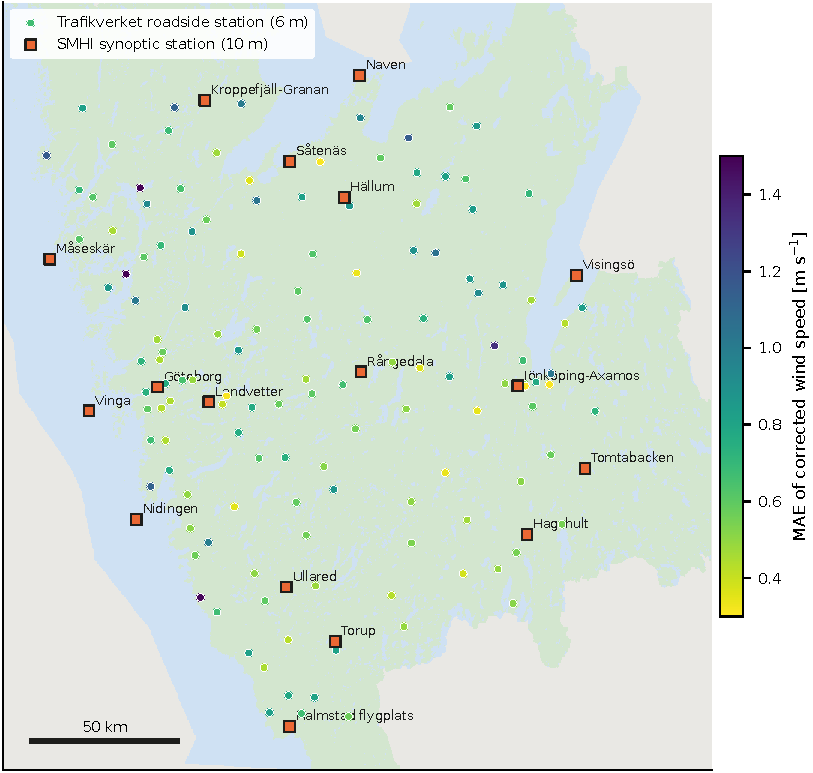
\includegraphics[width=0.85\textwidth]{figures/fig02_sweden_area.pdf}
\caption{Swedish check region: SMHI synoptic stations (squares), Trafikverket roadside stations (circles, coloured by the mean absolute error of the corrected wind speed) and road RV40.}
\label{fig:map-se}
\end{figure}

\begin{figure}[!htbp]
\centering
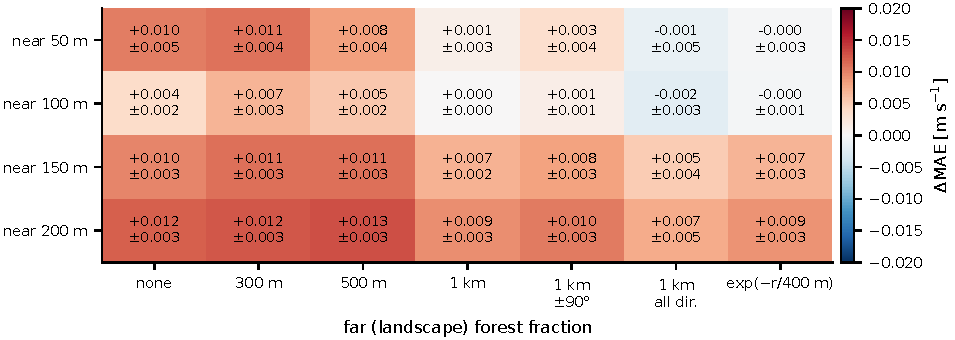
\includegraphics[width=\textwidth]{figures/fig07_two_shelter_scales_sweden.pdf}
\caption{Two shelter scales in the Swedish check region: cross-validated MAE difference ($\pm$ SE) for combinations of the near-tree radius and the landscape forest fraction, relative to \SI{100}{m} and \SI{1}{km}.}
\label{fig:twoscale}
\end{figure}

\begin{figure}[!htbp]
\centering
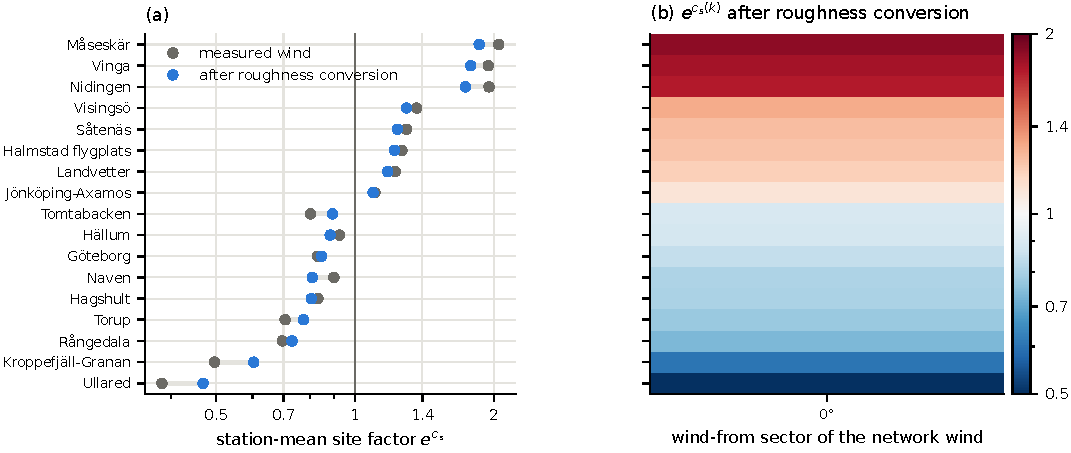
\includegraphics[width=0.8\textwidth]{figures/fig08_site_factors_sweden.pdf}
\caption{Site factors of the SMHI reference stations in the Swedish check region.}
\label{fig:site-se}
\end{figure}
